\documentclass[oneside, final, 10pt]{extarticle}
\usepackage[utf8]{inputenc}
\usepackage[russian]{babel}
\usepackage{vmargin}
\usepackage{listings}
\usepackage{graphicx}
\DeclareGraphicsRule{*}{mps}{*}{}
%\usepackage{ucs}
\setpapersize{A4}
\setmarginsrb{2cm}{2cm}{2cm}{2cm}{0pt}{0mm}{0pt}{13mm}
\usepackage{indentfirst}		%красная строка
%\usepackage{color}
\sloppy

\begin{document}
\begin{titlepage}
	\begin{centering}
		\textsc{Министерство образования и науки Российской Федерации}\\
		\textsc{Новосибирский государственный технический университет}\\
		\textsc{Кафедра теоритической и прикладной информатики}\\
	\end{centering}
	%\centerline{\hfill\hrulefill\hrulefill\hfill}
	\vfill
	\vfill
	\vfill
	\Large
	\centerline{Практическая работа}
	\centerline{по дисциплине "<Технологии разработки программного обеспечения">}
	\centerline{\bfПриложение "<Конвертер систем счисления">}
	\normalsize
	\vfill
	\vfill
	\vfill
	\begin{flushleft}
		\begin{minipage}{0.3\textwidth}
			\begin{tabular}{l l}
				Факультет: & ПМИ\\
				Группа: & ПМИ-41\\
				Студент: & Кислицын И. О.\\
				Преподаватель: & Зайцев М. Г.
			\end{tabular}
		\end{minipage}
	\end{flushleft}
	\vfill
	\vfill
	\begin{centering}
		Новосибирск\\
		2017\\
	\end{centering}
\end{titlepage}
\setcounter{page}{2}
\lstset{
	breaklines=\true,
	%frame=single,
	basicstyle=\footnotesize\ttfamily,
	tabsize=2,
	showspaces=\false,
	breaklines=\true,
	breakatwhitespace=\true,
	%escapeinside={"}{"},
	%inputencoding=utf8x,
	extendedchars=\true,
	keepspaces=\true
}
\section{Цель работы}

Объектно-ориентированный анализ, проектирование и реализация приложения "<Конвертер систем счисления"> для преобразования действительных чисел представленных в системе счисления с основанием \(p_1\) в действительные числа представленные в системе счисления с основанием \(p_2\).

\section{Ход работы}

\subsection{Класс Конвертер (Converter)}

\subsubsection{Описание}

Преобразователь действительных чисел из одной системы счисления в другую.

\subsubsection{Текст программы}

\lstset{caption=converter.js}
\lstinputlisting{./js/converter.js}

\subsubsection{Тестирование}
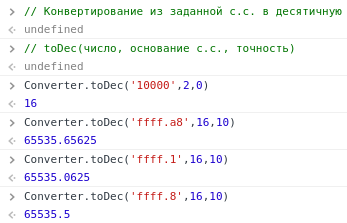
\includegraphics{./screen/test_converter_todec}
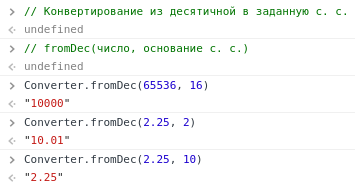
\includegraphics{./screen/test_converter_fromdec}
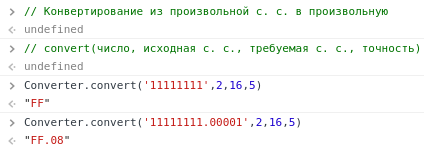
\includegraphics{./screen/test_converter_convert}

\subsection{Класс Редактор (Editor)}

\subsubsection{Описание}

Редактор чисел с заданным основанием.

Хранит строковое представление числа в заданной системе счисления. Обеспечивает добавление и удаление цифр числа, добавление разделителя целой и дробной части, отчистку (установку нулевого значения), чтение числа из строки.

\subsubsection{Текст программы}

\lstset{caption=editor.js}
\lstinputlisting{./js/editor.js}

\subsubsection{Тестирование}
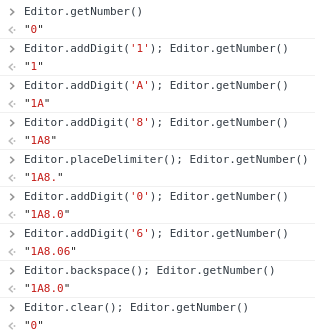
\includegraphics{./screen/test_editor}

\subsection{Класс История (History)}

\subsubsection{Описание}

Документирование операций перевода чисел из одной системы счисления в другую.

\subsubsection{Текст программы}

\lstset{caption=history.js}
\lstinputlisting{./js/history.js}

\subsubsection{Тестирование}
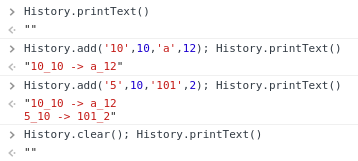
\includegraphics{./screen/test_history}

\subsection{Класс Управление (Runtime)}

\subsubsection{Описание}

Единственный метод класса (\verb`init()`) вызывается, когда графический интерфейс приложения загружен. Связывает событи графического интерфейса приложения с методами класса IFace.

\subsubsection{Текст программы}

\lstset{caption=runtime.js}
\lstinputlisting{./js/runtime.js}

\subsection{Класс Интерфейс (IFace)}

\subsubsection{Описание}

Данный класс связывает пользовательский интерфейс (HTML-layer) и остальные классы. Его методы обеспечивают управление визуальными элементами (например, включение и отключение ненужных кнопок для ввода цифр при смене основания системы счисления).

\subsubsection{Текст программы}

\lstset{caption=iface.js}
\lstinputlisting{./js/iface.js}

\subsubsection{Тестирование}
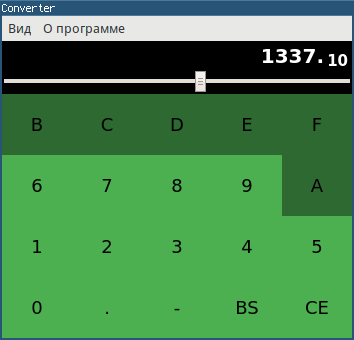
\includegraphics{./screen/test_iface1}
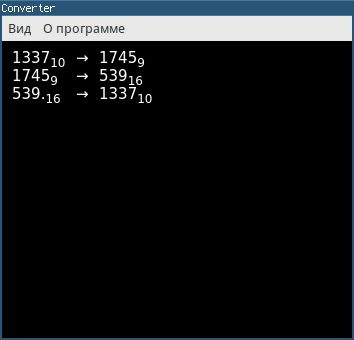
\includegraphics{./screen/test_iface2}
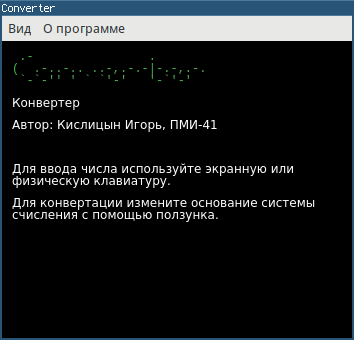
\includegraphics{./screen/test_iface3}

\subsection{Класс About}

\subsubsection{Описание}

Хранит справочную информацию о приложении.

\subsubsection{Текст программы}

\lstset{caption=about.js}
\lstset{escapeinside={ru}{ur}}
\lstinputlisting{./js/about.js}

\subsection{Диаграмма классов}
\includegraphics{./uml/class.1}

\subsection{Usecase-диаграмма}
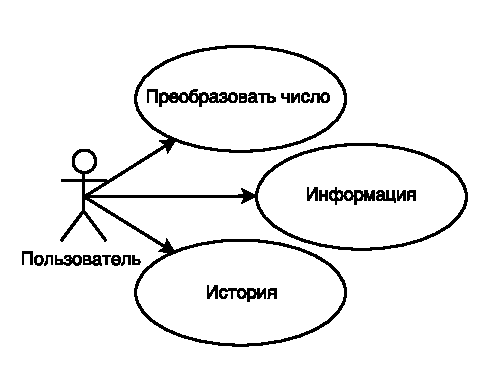
\includegraphics{./uml/usecase}

\subsection{Диаграмма последовательности}
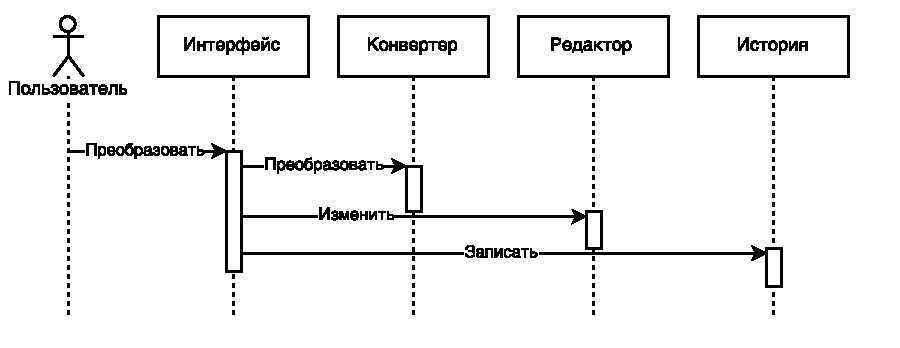
\includegraphics{./uml/seq_convert}

\end{document}
